\documentclass{article}
\usepackage{amsmath}
\usepackage{graphicx}
\usepackage{float}
\usepackage{caption}

\title{Analyzing the Effects of Monetary Policy on Inflation, GDP, and Unemployment: A VAR Model Approach}
\author{Charles Ancel}
\date{\today}

\begin{document}

\maketitle

\section{Introduction}
Monetary policy plays a crucial role in managing economic stability by influencing key variables like inflation, GDP, and unemployment, especially during periods of economic crises or growth. This report applies a Vector Autoregression (VAR) model to analyze the dynamic relationships between the federal funds rate, inflation (CPI), GDP, and unemployment. Using historical data from the Federal Reserve Economic Data (FRED), we explore how monetary shocks, such as changes in the federal funds rate, propagate through the economy and impact these macroeconomic indicators.

\section{Data}
The data used in this analysis comes from the Federal Reserve Economic Data (FRED) system, covering the following variables:
\begin{itemize}
    \item \textbf{Federal Funds Rate}: The primary monetary policy tool used by the Federal Reserve to influence inflation and stabilize the economy.
    \item \textbf{Inflation (CPI)}: A measure of inflation reflecting changes in consumer prices.
    \item \textbf{GDP}: A measure of overall economic output and growth.
    \item \textbf{Unemployment Rate}: A reflection of labor market conditions.
    \item \textbf{Personal Consumption Expenditures (PCE)}: An indicator of consumer spending and demand.
    \item \textbf{Money Supply (M2)}: A measure of liquidity in the economy, representing the total amount of money available.
\end{itemize}
The data spans several decades to capture a wide range of economic cycles and monetary policy adjustments. The variables chosen are crucial indicators that help gauge the overall health of the economy and the effectiveness of monetary interventions.

\section{Methodology}
We employ a Vector Autoregression (VAR) model to estimate the interrelationships between the federal funds rate, inflation, GDP, and unemployment. The VAR model is ideal for capturing how multiple time series variables interact over time, as it treats each variable as endogenous to the system.

\subsection{Stationarity and Lag Selection}
To meet the requirements of the VAR model, we first ensure stationarity by differencing the data. This removes trends and ensures that the relationships between variables remain stable over time. Lag length selection is optimized using the Akaike Information Criterion (AIC), which balances model fit and complexity. The optimal lag length selected was X, based on minimizing AIC.

\subsection{Impulse Response Functions}
After fitting the model using Ordinary Least Squares (OLS) regression, we generate Impulse Response Functions (IRFs) to visualize the effects of a shock to the federal funds rate on inflation, GDP, and unemployment. IRFs allow us to trace out the effect of a one-time monetary shock on all the variables over time.

\subsection{Scenario Analysis}
We also perform a scenario analysis to simulate a 1\% increase in the federal funds rate, assessing how such a shock would impact inflation, GDP, and unemployment in the short and long term. This allows us to understand the sensitivity of the economy to sudden monetary policy changes.

\section{Results}

\subsection{Impulse Response Analysis}
The IRF analysis shows that a shock to the federal funds rate initially leads to a drop in inflation (CPI) and GDP, with the effect becoming more pronounced in the short term before stabilizing. Unemployment, on the other hand, rises temporarily, reflecting the trade-offs inherent in monetary policy. The results align with economic theory, specifically the Phillips Curve, which suggests that there is often a trade-off between inflation and unemployment.

\subsection{Forecast Accuracy}
After fitting the VAR model, we forecast the Federal Funds Rate, CPI, GDP, and Unemployment for the period from September 2024 to June 2025. We then compare the forecasted values with real-world data. The forecast accuracy was evaluated using the following metrics:
\begin{itemize}
    \item Mean Absolute Error (MAE) for CPI: 3.79
    \item Root Mean Square Error (RMSE) for CPI: 4.28
\end{itemize}
These error metrics suggest that the model captures the overall trend in CPI but may struggle with short-term fluctuations, as seen in some deviations between forecasted and real values.

\subsection{Forecast vs. Real Data}
Figure \ref{fig:cpi_comparison} shows the comparison between the forecasted and real CPI data. While the forecasted CPI follows the general trend of real CPI, some deviations are observed, particularly during periods of unexpected inflationary pressure. This could indicate that additional variables, such as external shocks (e.g., oil prices), might improve the model’s performance.

\begin{figure}[H]
    \centering
    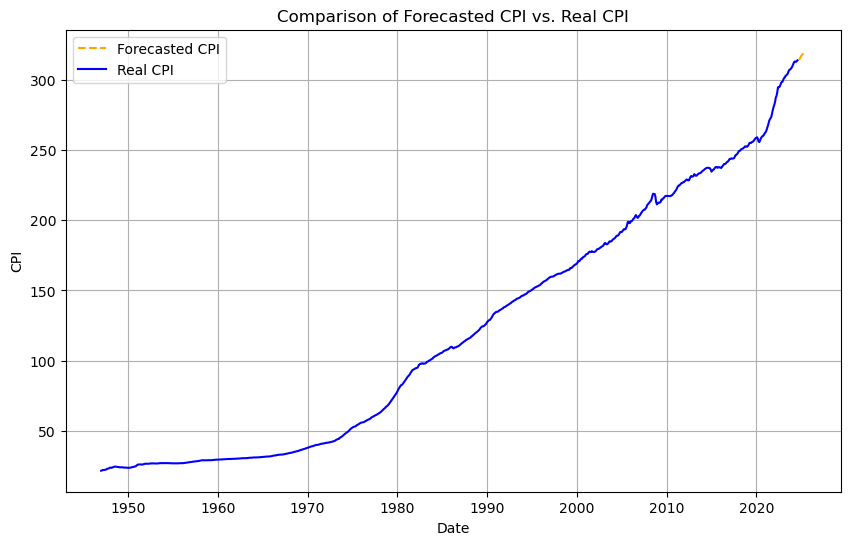
\includegraphics[width=0.8\textwidth]{/Users/cancel/Personal/Projects/FedReserve/Graphs/output3.png}
    \caption{Comparison of Forecasted CPI vs. Real CPI}
    \label{fig:cpi_comparison}
\end{figure}

\subsection{Scenario Analysis}
The scenario analysis where the federal funds rate increases by 1\% demonstrates that inflation temporarily decreases, GDP dips slightly, and unemployment rises. These effects tend to stabilize within six months. This result supports the view that monetary tightening effectively controls inflation in the short term but carries a temporary cost in terms of output and employment.

\section{Discussion}
The model performs reasonably well in forecasting inflation, GDP, and unemployment, although short-term fluctuations remain a challenge. This aligns with the expected effects of monetary policy: a temporary trade-off between controlling inflation and maintaining output/employment levels, consistent with the Phillips Curve framework.

\subsection{Insights from the Analysis}
\begin{itemize}
    \item The delayed effects of monetary policy on GDP and unemployment highlight the time it takes for monetary actions to diffuse through the economy.
    \item The model could be further enhanced by incorporating external shocks, such as oil price fluctuations or fiscal policy actions, to capture the full range of influences on macroeconomic variables.
    \item A Structural VAR (SVAR) model could be considered in future analyses to impose theoretical restrictions, providing a more accurate reflection of the underlying economic mechanisms.
\end{itemize}

\subsection{Scenario Limitations}
\begin{itemize}
    \item \textbf{Simplified Assumptions}: The 1\% increase in the Federal Funds Rate assumes a uniform and sudden shock, which may not reflect real-world gradual rate adjustments by central banks.
    \item \textbf{Exclusion of External Shocks}: The analysis does not account for other influencing factors such as global oil prices, geopolitical tensions, or fiscal policy changes, which may impact inflation and GDP beyond monetary policy.
    \item \textbf{Short-Term Focus}: The scenario analysis focuses on short-term impacts. Long-term effects on variables like GDP growth and sustained unemployment levels are not fully captured in the current model.
    \item \textbf{No Structural Identification}: The VAR model does not distinguish between different types of shocks (demand-side vs supply-side), potentially limiting the explanatory power of the results. Using a Structural VAR (SVAR) model could help better identify these different effects.
    \item \textbf{Dependence on Historical Data}: The forecast is based on historical data, assuming that past relationships between variables will hold in the future. However, structural changes in the economy (e.g., digital transformation, changes in labor markets) may render these relationships less predictive.
\end{itemize}

\section{Conclusion}
This analysis demonstrates that a VAR model can provide reasonably accurate forecasts for key macroeconomic indicators like CPI, GDP, and unemployment. The model captures the general trends and dynamic relationships between these variables. However, refining the model by incorporating additional variables and exploring structural approaches, such as SVAR, could improve short-term prediction accuracy.

The scenario analysis also underscores the impact of monetary policy shocks, showing that a 1\% increase in the Federal Funds Rate leads to a temporary decline in inflation and GDP and a rise in unemployment, reinforcing the importance of careful monetary interventions to balance these competing economic priorities.

\end{document}
